\documentclass{article}
\usepackage[MeX]{polski}
\usepackage{parskip}
\usepackage[utf8]{inputenc}
\usepackage{graphicx}
\title{Messim - Programowanie }
\author{\textsc{Paweł Sołtysiak I1-41A} \\ \texttt{psoltysiak@wi.zut.edu.pl}}
\begin{document}
\maketitle

\section{Opis}
Aplikacja 
\section{Prezentacja działania aplikacji}
Strona główna dla użytkownika niezalogowanego

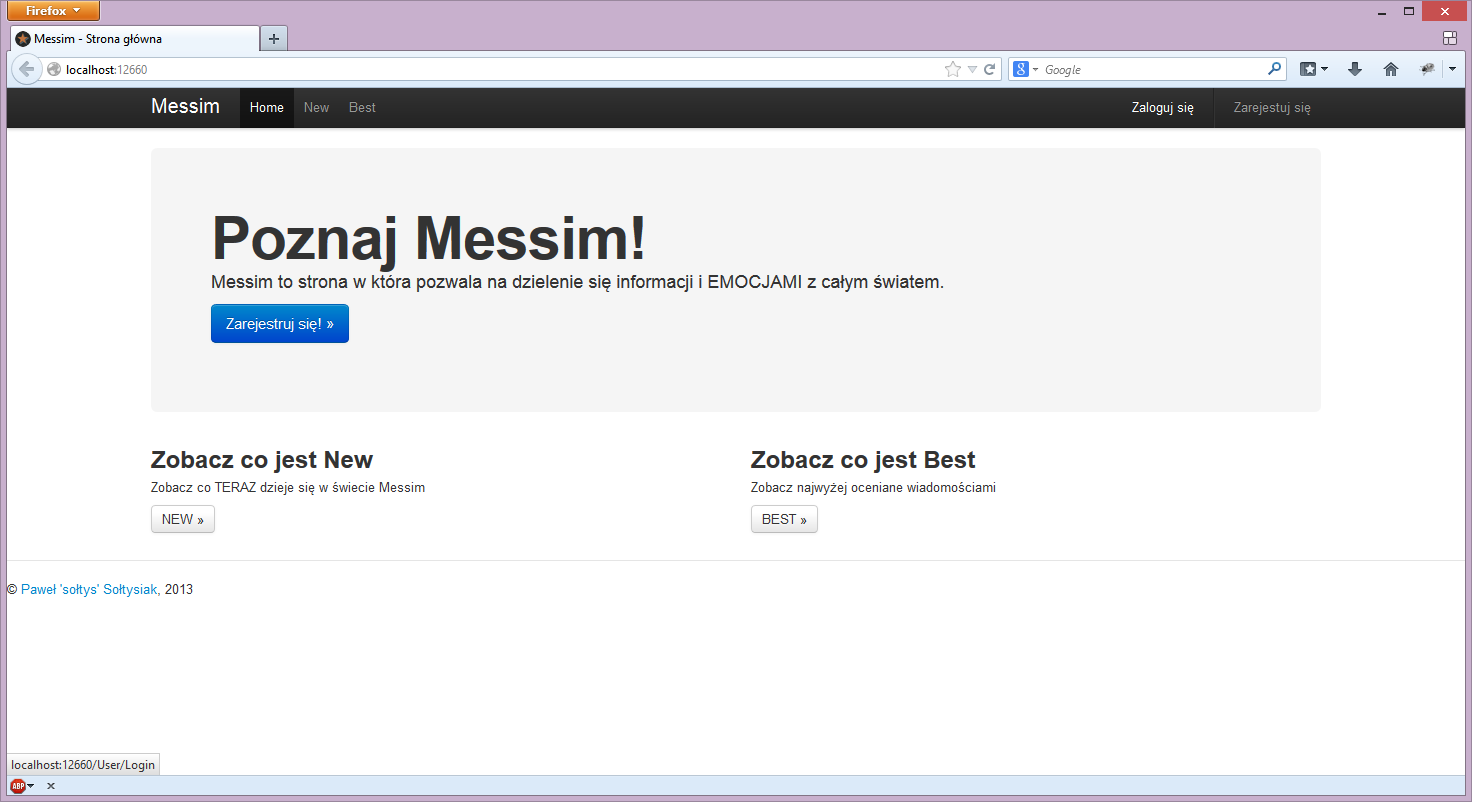
\includegraphics[width=\textwidth]{screenshots/home_page_not_singup}

Formularz rejestracji

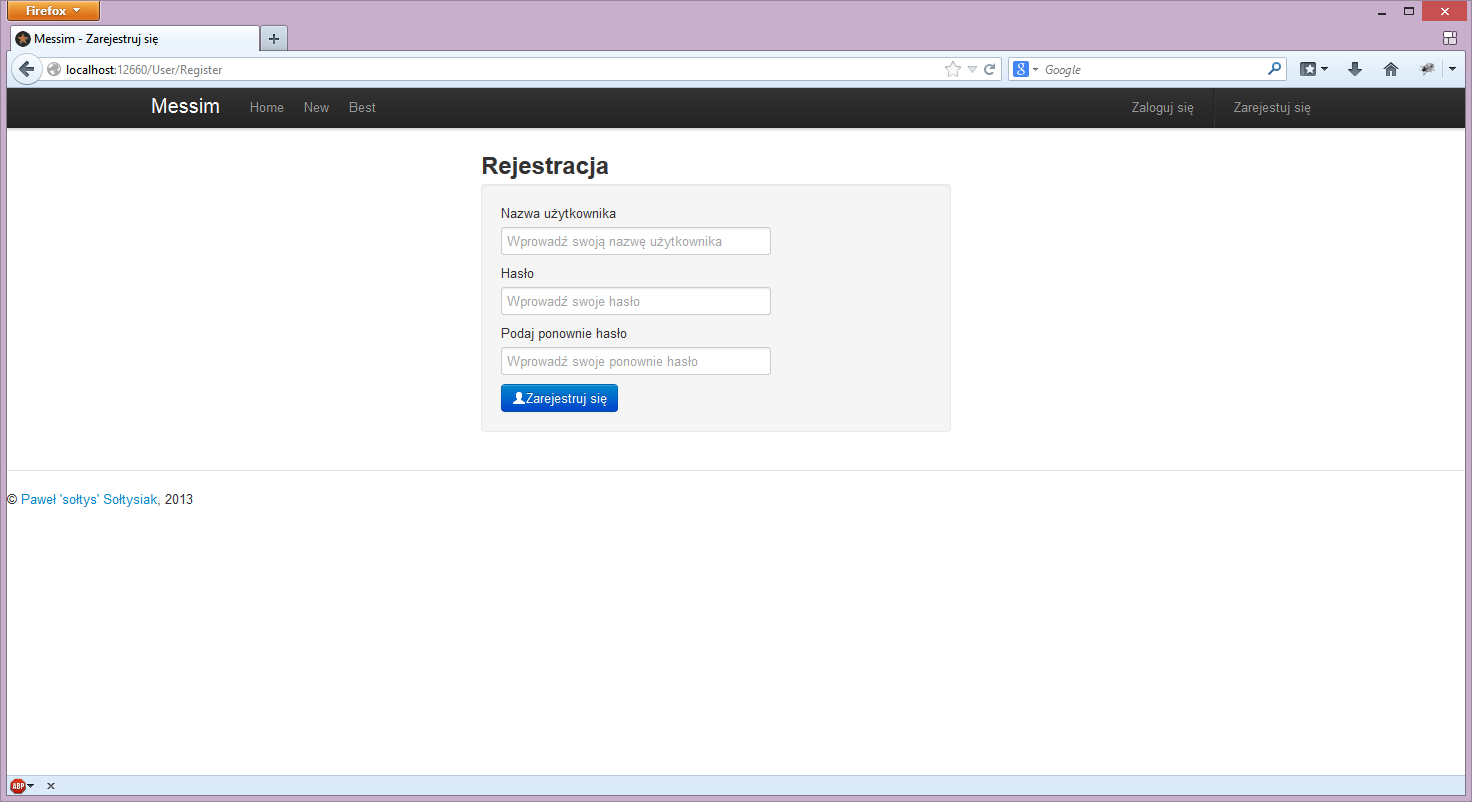
\includegraphics[width=\textwidth]{screenshots/register_page}

Strona główna dla użytkownika zalogowanego

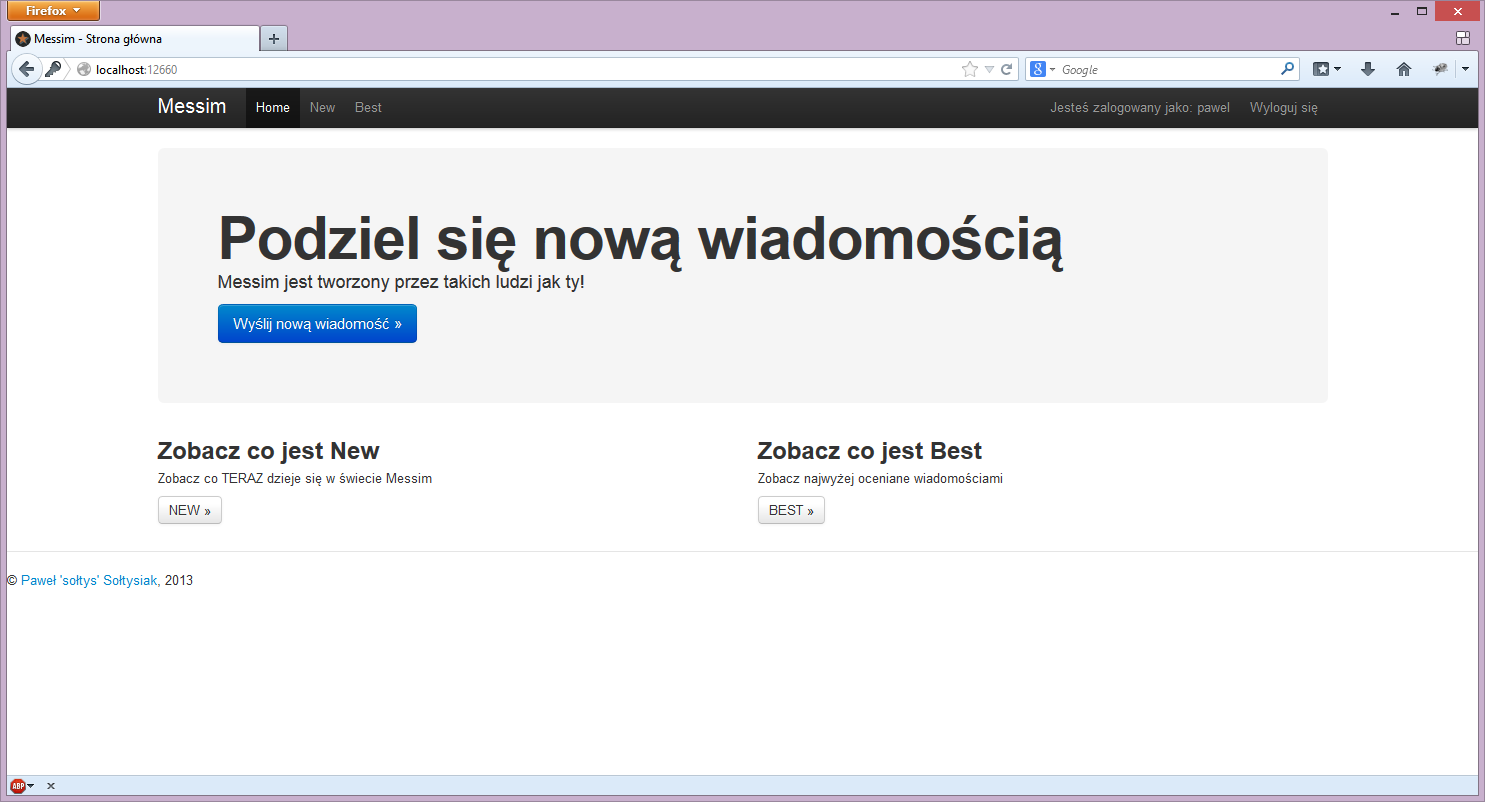
\includegraphics[width=\textwidth]{screenshots/home_page_with_user}

Formularz do przesyłania wiadomości i zdjęć

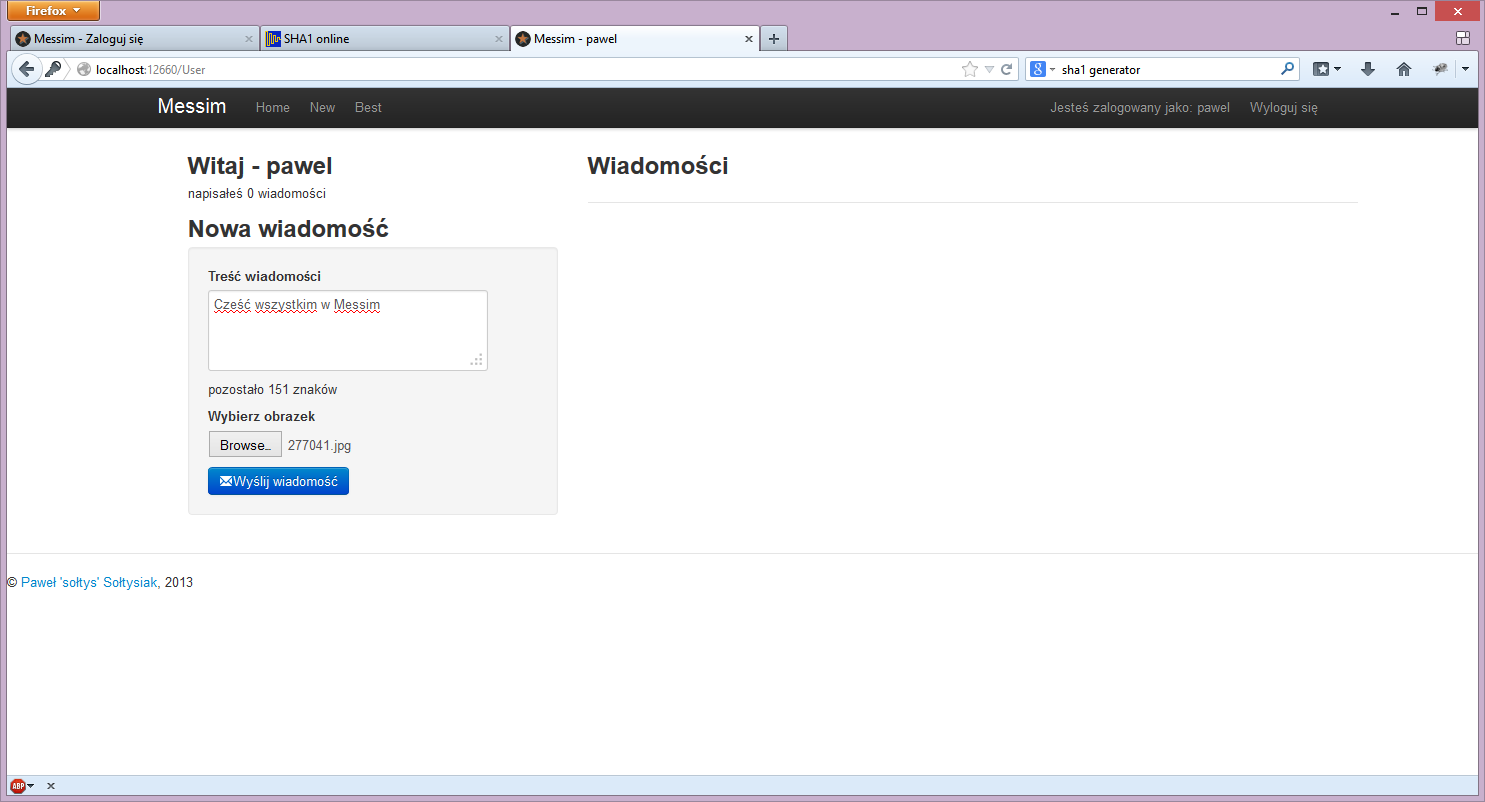
\includegraphics[width=\textwidth]{screenshots/posting_first_image}

Profil osoby po wysłaniu zdjęcia

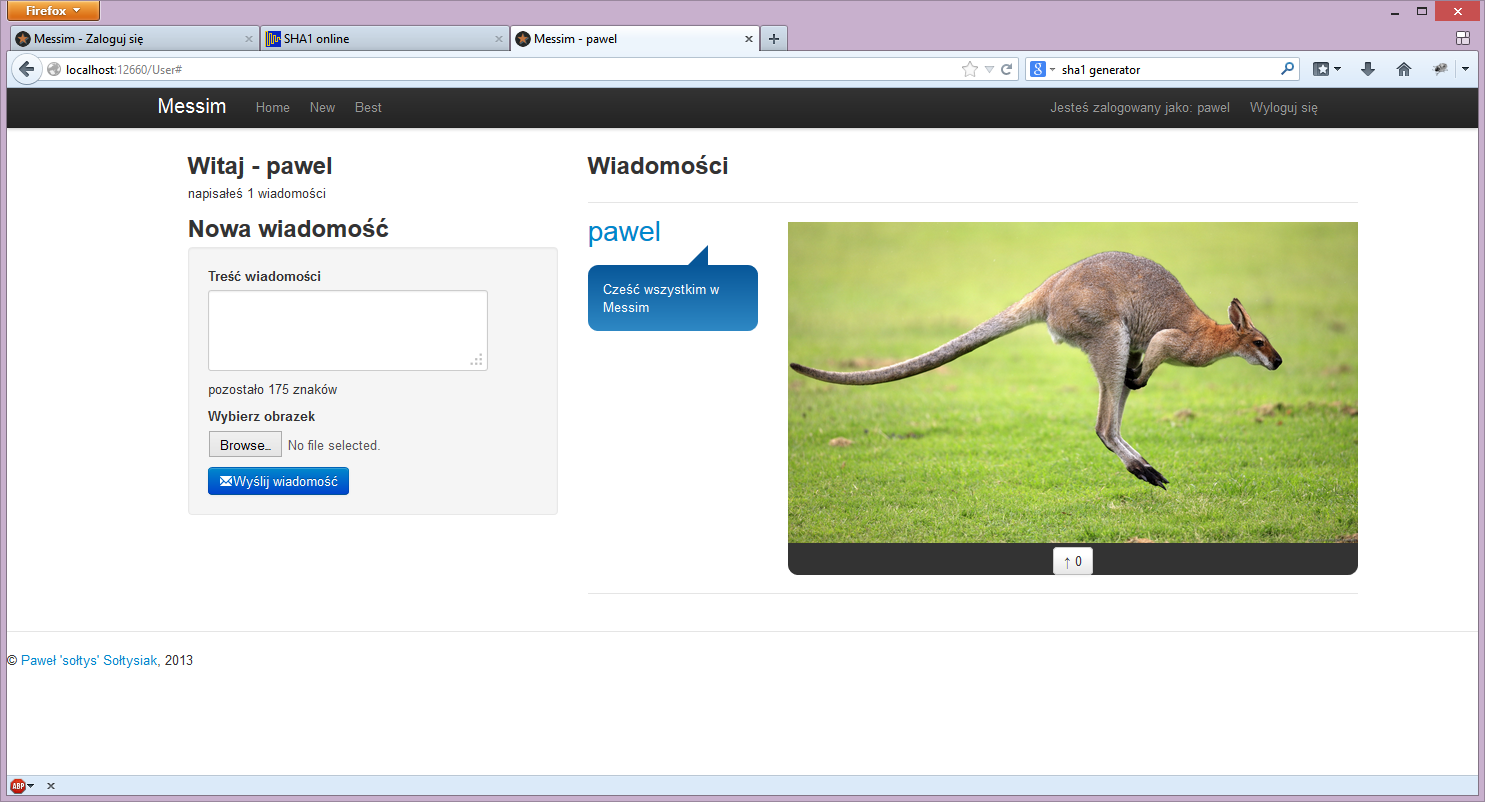
\includegraphics[width=\textwidth]{screenshots/posted_first_image}

\section{Opis technologiczny}
\begin{itemize}
\item Język programowania \texttt{C\#}
\item .NET Framework 4.0
\item ASP.NET MVC 3.0
\item Entity Framework
\item NUnit
\end{itemize}
\section{Informacje dodatkowe}

Z swoich starych projektów wyciągnąłem projekt aplikacji internetowej. Strona była tworzona z myślą o pokazaniu jej na tzw. "Nocy z Microsoft" gdzie grupy studenckie .NET z całego kraju przyjeżdżają aby pokazać która grupa jest najlepsza.

\end{document}

